\documentclass[aspectratio=169, t, 8pt]{beamer}

%------configurando acentos-----------
\usepackage[utf8]{inputenc}
\usepackage[brazil]{babel}

\usepackage{graphicx}

%-------Estilos Beamer---------------
\usetheme{metropolis}
%\usecolortheme{crane}
%coment
%\usefonttheme{serif}
\linespread{1.2}

% Personalização de Cores (Exemplo: Minimal Teal)
% Cores Base
\definecolor{BgCanvas}{HTML}{F9F9FB}      % Off-white muito suave
\definecolor{MainText}{HTML}{2B2D42}      % Grafite escuro para alta legibilidade
\definecolor{PrimaryAccent}{HTML}{4A6FA5} % Az
\definecolor{SunCoastFg}{HTML}{F2A154}
% --- CONFIGURAÇÕES DE TEMA BEAMER ---
%\usetheme{metropolis}

\setbeamertemplate{itemize item}{\textcolor{MainText}{$\bullet$}}
\setbeamertemplate{itemize subitem}{\textcolor{MainText}{\scriptsize$\circ$}}
\setbeamertemplate{itemize 3rditem}{\textcolor{MainText}{\tiny$\blacksquare$}}

\setbeamercolor{background canvas}{bg=BgCanvas}
\setbeamercolor{normal text}{fg=MainText}
\setbeamercolor{frametitle}{bg=SunCoastFg, fg=BgCanvas}
\setbeamercolor{title}{fg=MainText}
\setbeamercolor{subtitle}{fg=PrimaryAccent}
\setbeamercolor{structure}{fg=PrimaryAccent}

% Remove a linha amarela padrão do Metropolis sob o título
\setbeamertemplate{title separator}{}
\setbeamertemplate{progress bar in section page}{}


%--------Dados do Documento
\title{Matemática: Lista de Exercícios}
\author{prof. Eduardo}
\institute{Pré-Universitário Oficina do Saber / UFF}
\date{\today}


%-------- Pacotes Matemática -------------
\usepackage{amsmath}
\usepackage{amsthm}
\usepackage{amsfonts}
\usepackage{amssymb}
\usepackage{xfrac}
\usepackage{thmtools}

%-------- Configuração Listas---------
% \usepackage{enumitem}
\usepackage[inline]{enumitem}

\setcounter{tocdepth}{2}

\newcounter{questaovest}
\newcommand{\vest}[1]{\stepcounter{questaovest}\item[\textbf{Questão \arabic{questaovest}} (#1):]}
\setlist[enumerate]{
    align=left,
    leftmargin=1.8em,
    itemindent=1.8em
    }

\setlist[enumerate,2]{
    label=\alph*.,
    font=\bfseries,
    itemsep=0.1pt,
    labelsep=0em,
    parsep=0pt,
    leftmargin=0em,
    }

%------------- Atalho para imagens ------------
\graphicspath{{../../src/img/semana10/}}


\begin{document}

\begin{frame} %capa
        \vspace*{\fill}
            
            \begin{columns}[c]
                \begin{column}{0.5\textwidth}
                    {\usebeamerfont{title}\usebeamercolor[fg]{title}\inserttitle}\vspace{0.2cm}
                    
                    {\usebeamerfont{subtitle}\usebeamercolor[fg]{subtitle}\insertsubtitle}\vspace{0.5cm}

                {\usebeamerfont{author}\insertauthor}\vspace{0.3cm}

                {\usebeamerfont{institute}\insertinstitute}\vspace{0.3cm}

                {\usebeamerfont{date}\insertdate}
            \end{column}
            
            
            \begin{column}{0.4\textwidth}
                \centering
                
\includegraphics[width=0.4\textwidth]{../logo_ofSaber.png}

                \vspace{.4cm}
                \vspace*{\fill}
        \begin{columns}[c]
            \begin{column}{.5\textwidth}
                \centering
\includegraphics[width=.5\textwidth]{../Proex02c.png}
            \end{column}
            \begin{column}{.5\textwidth}
                \centering
\includegraphics[width=0.4\textwidth]{../Logo_UFF.png}
            \end{column}
        \end{columns}
        \vspace*{\fill}
            \end{column}
        \end{columns}
    \vspace*{\fill}
    \end{frame}
    
        % {
        %     \usebackgroundtemplate{
        %     \includegraphics[width=\paperwidth]{slide_02_contracapa.png}}
        %     \begin{frame}[plain]                
        %     \end{frame}
        % }


    \begin{frame} %Questão 01-D
        \frametitle{Funções}
        \vspace{-1.2em}
        \begin{enumerate}
            \begin{columns}
                \begin{column}{.9\textwidth}
                    \vest{UFRGS-2010}Em fevereiro, o governo da Cidade do México, metrópole com uma das maiores frotas de automóveis do mundo, passou a oferecer à população bicicletas como opção de transporte. Por uma anuidade de 24 dólares, os usuários têm direito a 30 minutos de uso livre por dia. O ciclista pode retirar em uma estação e devolver em qualquer outra e, se quiser estender a pedalada, paga 3 dólares por hora extra.
                    \vspace{1em}
                    A expressão que relaciona o valor f pago pela utilização da bicicleta por um ano, quando se utilizam $x$ horas extras nesse período é

                    \begin{enumerate}[label=\alph*.)]
                        \item $f(x) = 3x$
                        \item $f(x) = 24$
                        \item $f(x) = 27$
                        \item $f(x) = 3x + 24$
                        \item $f(x) = 24x + 3$
                    \end{enumerate}
                \end{column}
            \end{columns}
        \end{enumerate}
    \end{frame}

    \begin{frame}{Funções} %E
        \begin{columns}[totalwidth=.9\textwidth]
            \begin{column}{\textwidth}
                \begin{enumerate}
                    \vest{IFAL-2017} Em uma partida de futebol, a trajetória vertical de uma bola lançada por um jogador segue a função $h(t) = 8t - 2t^2$, onde $h$ representa a altura da bola em metros em relação ao solo e $t$ é o tempo decorrido em segundos após o chute. Pede-se para determinar a altura máxima atingida pela bola.

                    \begin{enumerate}
                        \item 2 m.
                        \item 4 m.
                        \item 6 m.
                        \item 8 m.
                        \item 10 m.
                    \end{enumerate}
                \end{enumerate}
            \end{column}
        \end{columns}
    \end{frame}

    \begin{frame}{Contagem} %D
        \begin{columns}[totalwidth=.9\textwidth]
            \begin{column}{\textwidth}
                \begin{enumerate}
                    \vest{UFPE-2015} A prova final de Geografia de uma escola é composta de 10 itens com alternativas do tipo “verdadeiro ou falso”. De quantas maneiras diferentes um estudante poderá responder esta prova, de forma que ele só assinale apenas uma alternativa em cada questão?

                    \vspace{1.2em}

                    \begin{enumerate}[label=\alph*)]
                        \item 20
                        \item 64
                        \item 256
                        \item 512
                        \item 1024
                    \end{enumerate}
                \end{enumerate}
            \end{column}
        \end{columns}
    \end{frame}

    \begin{frame}{Geometria}
      \begin{columns}[totalwidth=.9\textwidth]
        \begin{column}{\textwidth}
            \begin{enumerate}
                \vest{CEFET/RJ-2017} Uma fita de papel retangular é dobrada conforme a figura a seguir.

                \vspace{1.2em}

                \begin{columns}[totalwidth=\textwidth,T]
                    \begin{column}{.45\textwidth}
                        \centering
                        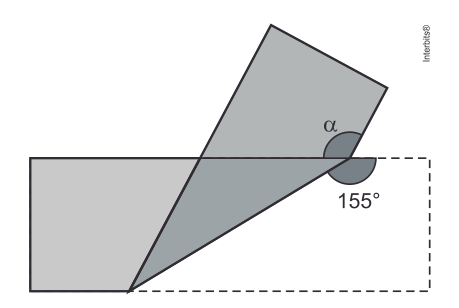
\includegraphics[width=\textwidth]{questao_angulo.png}
                    \end{column}
                    \begin{column}{.45\textwidth}
                       O valor do ângulo $\alpha$ marcado na figura é:
                        
                        \vspace{1em}

                        \raggedright
                        \begin{minipage}{.8\textwidth}
                            \begin{enumerate*}[itemjoin={\hfill}]
                                \item $155^{\circ}$
                                \item $150^{\circ}$
                                \item $140^{\circ}$
                                \item $130^{\circ}$
                            \end{enumerate*}
                        \end{minipage}
                    \end{column}
                \end{columns}
            \end{enumerate}
        \end{column}
      \end{columns}  
    \end{frame}

    \begin{frame}{Contagem}
        \begin{columns}[totalwidth=.9\textwidth]
            \begin{column}{\textwidth}
                \begin{enumerate}
                    \vest{FATEC-1999} (Uece 2015) No colégio municipal, em uma turma com 40 alunos, 14 gostam de Matemática, 16 gostam de Física, 12 gostam de Química, 7 gostam de Matemática e Física, 8 gostam de Física e Química, 5 gostam de Matemática e Química e 4 gostam das três matérias. Nessa turma, o número de alunos que não gostam de nenhuma das três disciplinas é

                    \vspace{1.2em}

                    \begin{columns}[totalwidth=\textwidth]
                        \begin{column}{\textwidth}
                            \centering
                            \begin{minipage}{.7\textwidth}
                                \begin{enumerate*}[itemjoin={\hfill}]
                                    \item $6$
                                    \item $9$
                                    \item $12$
                                    \item $14$
                                \end{enumerate*}
                            \end{minipage}
                        \end{column}
                    \end{columns}
                \end{enumerate}
            \end{column}
        \end{columns}
    \end{frame}
\end{document}